\documentclass[a4paper,oneside,DIV=10,12pt]{scrartcl}

\usepackage{graphicx}
\usepackage{float}

\usepackage{fontspec}
\setmainfont{STIX Two Text}
%\setsansfont{Roboto}
\newfontfamily{\cyrillicfontsf}{Roboto}

\usepackage{microtype}

\usepackage{polyglossia}
\setmainlanguage{ukrainian}

\usepackage{amsmath}
\usepackage{unicode-math}
\setmathfont{STIX Two Math}
\usepackage[retainorgcmds]{IEEEtrantools}

\usepackage{booktabs}

\usepackage{siunitx}
\sisetup{output-decimal-marker = {,},
exponent-product = {\cdot}}

\newcommand\schel[1]{\textit{#1}}

\begin{document}
	\begin{titlepage}
		\begin{center}
			Міністерство освіти і науки України\\
			Національний авіаційний університет\\
			Навчально-науковий інститут комп'ютерних інформаційних технологій\\
			Кафедра комп'ютеризованих систем управління
			
			\vspace{\fill}
				Лабораторна робота №4\\
				з дисципліни «Теорія електричних та магнітних кіл»\\
				на тему: «Розрахунок складного електричного~кола синусоїдного~струму з~експериментальною~перевіркою»\\
				Варіант №
				
			\vspace{\fill}
			
			\begin{flushright}
				Виконав:\\
				студент ННІКІТ СП-225\\
				Клокун Владислав\\
				Перевірив:\\
				Молчанов О.~В.
			\end{flushright}
			Київ 2017
		\end{center}
	\end{titlepage}
	
	\section{Мета роботи}
		\begin{enumerate}
			\item Набути необхідні навички практичного розрахунку складного електричного кола синусоїдного струму, використовуючи методи аналізу кіл.
			\item Перевірити правильність розрахунку кола, використовуючи рівняння балансу потужностей.
			\item Навчитися будувати векторну діаграму струмів та топографічну діаграму напруг контуру.
		\end{enumerate}
		
	\section{Короткі теоретичні відомості}
		Для розрахунку кіл змінного струму застосовують такі ж методи, що і для аналізу кіл постійного струму, а саме метод рівнянь Кірхгофа, методи контурних струмів, вузлових потенціалів, еквівалентних перетворень і т.п. Однак, ці методи аналізу можна застосовувати тільки в сукупності з теорією комплексних змінних.
		
		Відомо, що синусоїдні функції часу
		\[
			i(t) = I_m \sin(\omega t + \varphi_i), \quad
			u(t) = U_m \sin(\omega t + \varphi_i),
		\]
		якими описуються миттєві значення змінних струмів і напруг, можна представити у вигляді комплексних чисел:
		\[
			I_m = I_m e^{j \varphi_i}, \quad
			U_m = U_m e^{j \varphi_i},
		\]
		у яких.
	
	\section{Порядок виконання роботи}
		Для виконання даної лабораторної роботи можна використовувати лабораторний стенд №8 або скористатися магазинами резисторів, індуктивностей та ємностей. Але в будь-якому випадку необхідно зібрати вимірювальну частину схеми, зображеної на рисунку~\ref{fig:schematic-01} і по черзі провести необхідні вимірювання, підключаючи до виходу схеми елементи, вказані в таблиці~\ref{tab:measurement-01}.
		
		\begin{figure}[!htbp]
		\centering
			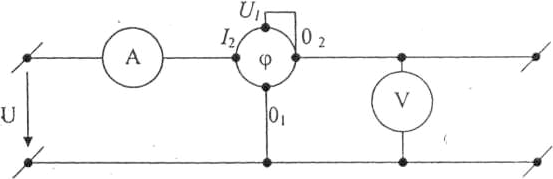
\includegraphics[width=0.7\textwidth]{schematic-01.png}
		\caption{Схема №1}
		\label{fig:schematic-01}
		\end{figure}
		
		\begin{table}[!htbp]
		\centering
			\begin{tabular}{
				l
				S
				S
				S
				S
				S
			}
				\toprule
					Параметри & {\schel{R1}} & {\schel{R2}} & {\schel{L}} & {\schel{R4}} & {\schel{C}} \\
				\midrule
					$U, \si{\volt}$         & {} & {} & {} & {} & {} \\
					$I, \si{\ampere}$       & {} & {} & {} & {} & {} \\
					$\varphi, \si{\degree}$ & {} & {} & {} & {} & {} \\
				\bottomrule
			\end{tabular}
		\caption{Дані №1}
		\label{tab:measurement-01}
		\end{table}
		
		Використовуючи дані таблиці~\ref{tab:measurement-01}, розрахувати значення активних опорів резисторів \schel{R1}, \schel{R2}, \schel{$R_{\text{К}}$}, \schel{R4}, \schel{$R_C$} і значення реактивних опорів індуктивності та ємності \schel{$X_{\text{К}}$}, \schel{$X_C$}. З'ясувати у викладача кількість джерел ЕРС, позначення та значення їх напруги у схемі, при яких необхідно розрахувати задане коло, і методи аналізу цього кола. Всі отримані дані занести у таблицю~\ref{}.
		
		\begin{table}[!htbp]
		\centering
			\begin{tabular}{
				S
				S
				S
				S
				S
				S
				S
				S
				S
				S
			}
				\toprule
					{$E_1, \si{\volt}$} &
					{$E_2, \si{\volt}$} &
					{$E_1, \si{\volt}$} &
					{$\schel{R1}, \si{\ohm}$} &
					{$\schel{R2}, \si{\ohm}$} &
					{$R_{\text{K}}, \si{\ohm}$} &
					{$X_{\text{К}}, \si{\ohm}$} &
					{$\schel{R4}, \si{\ohm}$} &
					{$R_C, \si{\ohm}$} &
					{$X_C, \si{\ohm}$}\\
				\midrule
					 & & & & & & & & & \\
				\bottomrule
			\end{tabular}
		\caption{Дані №2}
		\label{}
		\end{table}
		
		Розрахувати електричне коло на рисунку~\ref{fig:schematic-02} відповідно до завдання, використовуючи символічний метод розрахунку. Тобто необхідно визначити діючі значення струмів схеми заданими методами та діючі значення напруг на елементах кола. Перевірити правильність розрахунку кола за рівняннями балансу потужностей. Дані розрахунку занести в таблицю~\ref{tab:measurements-03}.
		
		\begin{figure}[!htbp]
		\centering
			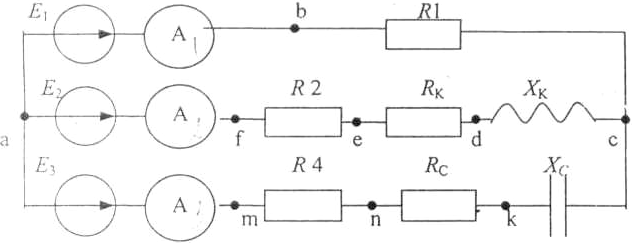
\includegraphics[width=\textwidth]{schematic-02.png}
		\caption{Схема №2}
		\label{fig:schematic-02}
		\end{figure}
		
		Зібрати електричну схему на рисунку~\ref{fig:schematic-02}, включивши в неї необхідні вимірювальні прилади. Виконати вимірювання струмів і напруг. Результати експерименту занести в таблицю~\ref{tab:measurements-03}.
		
		Використовуючи результати попередніх пунктів, обчислити похибку отриманих результатів. Результати обчислень занести в таблицю~\ref{tab:measurements-03}.
		
		Побудувати векторну діаграму струмів і топографічну діаграму напруг.
		
		\begin{table}[!htbp]
		\centering
			\begin{tabular}{
				l
				S
				S
				S
				S
				S
				S
				S
				S
				S
			}
				\toprule
					Метод &
					{$U$} &
					{$I_1$} &
					{$I_2$} &
					{$I_3$} &
					{$U_{bc}$} &
					{$U_{ce}$} &
					{$U_{ef}$} &
					{$U_{cn}$} &
					{$U_{nm}$} \\
				\midrule
					МКС     & & & & & & & & & \\
					МВП     & & & & & & & & & \\
					Дослід  & & & & & & & & & \\
					Похибка & & & & & & & & & \\
				\bottomrule
			\end{tabular}
		\caption{Дані №3}
		\label{tab:measurements-03}
		\end{table}
		
	\section{Висновки}
\end{document}